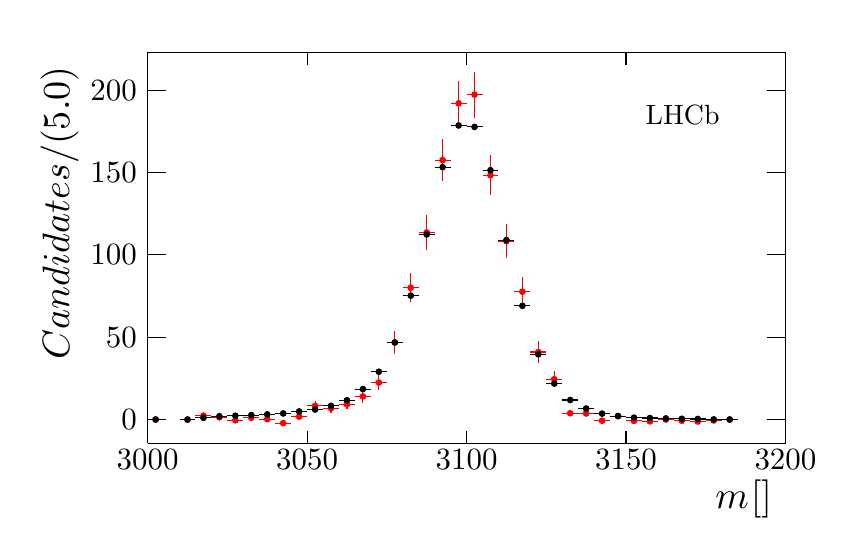
\begin{tikzpicture}
\pgfdeclareplotmark{cross} {
\pgfpathmoveto{\pgfpoint{-0.3\pgfplotmarksize}{\pgfplotmarksize}}
\pgfpathlineto{\pgfpoint{+0.3\pgfplotmarksize}{\pgfplotmarksize}}
\pgfpathlineto{\pgfpoint{+0.3\pgfplotmarksize}{0.3\pgfplotmarksize}}
\pgfpathlineto{\pgfpoint{+1\pgfplotmarksize}{0.3\pgfplotmarksize}}
\pgfpathlineto{\pgfpoint{+1\pgfplotmarksize}{-0.3\pgfplotmarksize}}
\pgfpathlineto{\pgfpoint{+0.3\pgfplotmarksize}{-0.3\pgfplotmarksize}}
\pgfpathlineto{\pgfpoint{+0.3\pgfplotmarksize}{-1.\pgfplotmarksize}}
\pgfpathlineto{\pgfpoint{-0.3\pgfplotmarksize}{-1.\pgfplotmarksize}}
\pgfpathlineto{\pgfpoint{-0.3\pgfplotmarksize}{-0.3\pgfplotmarksize}}
\pgfpathlineto{\pgfpoint{-1.\pgfplotmarksize}{-0.3\pgfplotmarksize}}
\pgfpathlineto{\pgfpoint{-1.\pgfplotmarksize}{0.3\pgfplotmarksize}}
\pgfpathlineto{\pgfpoint{-0.3\pgfplotmarksize}{0.3\pgfplotmarksize}}
\pgfpathclose
\pgfusepathqstroke
}
\pgfdeclareplotmark{cross*} {
\pgfpathmoveto{\pgfpoint{-0.3\pgfplotmarksize}{\pgfplotmarksize}}
\pgfpathlineto{\pgfpoint{+0.3\pgfplotmarksize}{\pgfplotmarksize}}
\pgfpathlineto{\pgfpoint{+0.3\pgfplotmarksize}{0.3\pgfplotmarksize}}
\pgfpathlineto{\pgfpoint{+1\pgfplotmarksize}{0.3\pgfplotmarksize}}
\pgfpathlineto{\pgfpoint{+1\pgfplotmarksize}{-0.3\pgfplotmarksize}}
\pgfpathlineto{\pgfpoint{+0.3\pgfplotmarksize}{-0.3\pgfplotmarksize}}
\pgfpathlineto{\pgfpoint{+0.3\pgfplotmarksize}{-1.\pgfplotmarksize}}
\pgfpathlineto{\pgfpoint{-0.3\pgfplotmarksize}{-1.\pgfplotmarksize}}
\pgfpathlineto{\pgfpoint{-0.3\pgfplotmarksize}{-0.3\pgfplotmarksize}}
\pgfpathlineto{\pgfpoint{-1.\pgfplotmarksize}{-0.3\pgfplotmarksize}}
\pgfpathlineto{\pgfpoint{-1.\pgfplotmarksize}{0.3\pgfplotmarksize}}
\pgfpathlineto{\pgfpoint{-0.3\pgfplotmarksize}{0.3\pgfplotmarksize}}
\pgfpathclose
\pgfusepathqfillstroke
}
\pgfdeclareplotmark{newstar} {
\pgfpathmoveto{\pgfqpoint{0pt}{\pgfplotmarksize}}
\pgfpathlineto{\pgfqpointpolar{44}{0.5\pgfplotmarksize}}
\pgfpathlineto{\pgfqpointpolar{18}{\pgfplotmarksize}}
\pgfpathlineto{\pgfqpointpolar{-20}{0.5\pgfplotmarksize}}
\pgfpathlineto{\pgfqpointpolar{-54}{\pgfplotmarksize}}
\pgfpathlineto{\pgfqpointpolar{-90}{0.5\pgfplotmarksize}}
\pgfpathlineto{\pgfqpointpolar{234}{\pgfplotmarksize}}
\pgfpathlineto{\pgfqpointpolar{198}{0.5\pgfplotmarksize}}
\pgfpathlineto{\pgfqpointpolar{162}{\pgfplotmarksize}}
\pgfpathlineto{\pgfqpointpolar{134}{0.5\pgfplotmarksize}}
\pgfpathclose
\pgfusepathqstroke
}
\pgfdeclareplotmark{newstar*} {
\pgfpathmoveto{\pgfqpoint{0pt}{\pgfplotmarksize}}
\pgfpathlineto{\pgfqpointpolar{44}{0.5\pgfplotmarksize}}
\pgfpathlineto{\pgfqpointpolar{18}{\pgfplotmarksize}}
\pgfpathlineto{\pgfqpointpolar{-20}{0.5\pgfplotmarksize}}
\pgfpathlineto{\pgfqpointpolar{-54}{\pgfplotmarksize}}
\pgfpathlineto{\pgfqpointpolar{-90}{0.5\pgfplotmarksize}}
\pgfpathlineto{\pgfqpointpolar{234}{\pgfplotmarksize}}
\pgfpathlineto{\pgfqpointpolar{198}{0.5\pgfplotmarksize}}
\pgfpathlineto{\pgfqpointpolar{162}{\pgfplotmarksize}}
\pgfpathlineto{\pgfqpointpolar{134}{0.5\pgfplotmarksize}}
\pgfpathclose
\pgfusepathqfillstroke
}
\definecolor{c}{rgb}{1,1,1};
\draw [color=c, fill=c] (0,0) rectangle (10,6.27517);
\draw [color=c, fill=c] (1.4,1.00403) rectangle (9.5,5.96141);
\definecolor{c}{rgb}{0,0,0};
\draw [c] (1.4,1.00403) -- (1.4,5.96141) -- (9.5,5.96141) -- (9.5,1.00403) -- (1.4,1.00403);
\definecolor{c}{rgb}{1,1,1};
\draw [color=c, fill=c] (1.4,1.00403) rectangle (9.5,5.96141);
\definecolor{c}{rgb}{0,0,0};
\draw [c] (1.4,1.00403) -- (1.4,5.96141) -- (9.5,5.96141) -- (9.5,1.00403) -- (1.4,1.00403);
\definecolor{c}{rgb}{1,0,0};
\draw [c,line width=0.4] (1.50125,1.30263) -- (1.50125,1.30542);
\draw [c,line width=0.4] (1.50125,1.30542) -- (1.50125,1.30821);
\draw [c,line width=0.4] (1.4,1.30542) -- (1.50125,1.30542);
\draw [c,line width=0.4] (1.50125,1.30542) -- (1.6025,1.30542);
\foreach \P in {(1.50125,1.30542)}{\draw[mark options={color=c,fill=c},mark size=2.402402pt,mark=*,mark size=1pt] plot coordinates {\P};}
\draw [c,line width=0.4] (1.90625,1.29609) -- (1.90625,1.3033);
\draw [c,line width=0.4] (1.90625,1.3033) -- (1.90625,1.31052);
\draw [c,line width=0.4] (1.805,1.3033) -- (1.90625,1.3033);
\draw [c,line width=0.4] (1.90625,1.3033) -- (2.0075,1.3033);
\foreach \P in {(1.90625,1.3033)}{\draw[mark options={color=c,fill=c},mark size=2.402402pt,mark=*,mark size=1pt] plot coordinates {\P};}
\draw [c,line width=0.4] (2.10875,1.32351) -- (2.10875,1.35585);
\draw [c,line width=0.4] (2.10875,1.35585) -- (2.10875,1.3882);
\draw [c,line width=0.4] (2.0075,1.35585) -- (2.10875,1.35585);
\draw [c,line width=0.4] (2.10875,1.35585) -- (2.21,1.35585);
\foreach \P in {(2.10875,1.35585)}{\draw[mark options={color=c,fill=c},mark size=2.402402pt,mark=*,mark size=1pt] plot coordinates {\P};}
\draw [c,line width=0.4] (2.31125,1.30958) -- (2.31125,1.33376);
\draw [c,line width=0.4] (2.31125,1.33376) -- (2.31125,1.35794);
\draw [c,line width=0.4] (2.21,1.33376) -- (2.31125,1.33376);
\draw [c,line width=0.4] (2.31125,1.33376) -- (2.4125,1.33376);
\foreach \P in {(2.31125,1.33376)}{\draw[mark options={color=c,fill=c},mark size=2.402402pt,mark=*,mark size=1pt] plot coordinates {\P};}
\draw [c,line width=0.4] (2.51375,1.28158) -- (2.51375,1.29593);
\draw [c,line width=0.4] (2.51375,1.29593) -- (2.51375,1.31029);
\draw [c,line width=0.4] (2.4125,1.29593) -- (2.51375,1.29593);
\draw [c,line width=0.4] (2.51375,1.29593) -- (2.615,1.29593);
\foreach \P in {(2.51375,1.29593)}{\draw[mark options={color=c,fill=c},mark size=2.402402pt,mark=*,mark size=1pt] plot coordinates {\P};}
\draw [c,line width=0.4] (2.71625,1.30607) -- (2.71625,1.32724);
\draw [c,line width=0.4] (2.71625,1.32724) -- (2.71625,1.34841);
\draw [c,line width=0.4] (2.615,1.32724) -- (2.71625,1.32724);
\draw [c,line width=0.4] (2.71625,1.32724) -- (2.8175,1.32724);
\foreach \P in {(2.71625,1.32724)}{\draw[mark options={color=c,fill=c},mark size=2.402402pt,mark=*,mark size=1pt] plot coordinates {\P};}
\draw [c,line width=0.4] (2.91875,1.30066) -- (2.91875,1.30973);
\draw [c,line width=0.4] (2.91875,1.30973) -- (2.91875,1.31879);
\draw [c,line width=0.4] (2.8175,1.30973) -- (2.91875,1.30973);
\draw [c,line width=0.4] (2.91875,1.30973) -- (3.02,1.30973);
\foreach \P in {(2.91875,1.30973)}{\draw[mark options={color=c,fill=c},mark size=2.402402pt,mark=*,mark size=1pt] plot coordinates {\P};}
\draw [c,line width=0.4] (3.12125,1.22885) -- (3.12125,1.25984);
\draw [c,line width=0.4] (3.12125,1.25984) -- (3.12125,1.29084);
\draw [c,line width=0.4] (3.02,1.25984) -- (3.12125,1.25984);
\draw [c,line width=0.4] (3.12125,1.25984) -- (3.2225,1.25984);
\foreach \P in {(3.12125,1.25984)}{\draw[mark options={color=c,fill=c},mark size=2.402402pt,mark=*,mark size=1pt] plot coordinates {\P};}
\draw [c,line width=0.4] (3.32375,1.31427) -- (3.32375,1.34164);
\draw [c,line width=0.4] (3.32375,1.34164) -- (3.32375,1.36902);
\draw [c,line width=0.4] (3.2225,1.34164) -- (3.32375,1.34164);
\draw [c,line width=0.4] (3.32375,1.34164) -- (3.425,1.34164);
\foreach \P in {(3.32375,1.34164)}{\draw[mark options={color=c,fill=c},mark size=2.402402pt,mark=*,mark size=1pt] plot coordinates {\P};}
\draw [c,line width=0.4] (3.52625,1.41873) -- (3.52625,1.47888);
\draw [c,line width=0.4] (3.52625,1.47888) -- (3.52625,1.53903);
\draw [c,line width=0.4] (3.425,1.47888) -- (3.52625,1.47888);
\draw [c,line width=0.4] (3.52625,1.47888) -- (3.6275,1.47888);
\foreach \P in {(3.52625,1.47888)}{\draw[mark options={color=c,fill=c},mark size=2.402402pt,mark=*,mark size=1pt] plot coordinates {\P};}
\draw [c,line width=0.4] (3.72875,1.39417) -- (3.72875,1.44886);
\draw [c,line width=0.4] (3.72875,1.44886) -- (3.72875,1.50354);
\draw [c,line width=0.4] (3.6275,1.44886) -- (3.72875,1.44886);
\draw [c,line width=0.4] (3.72875,1.44886) -- (3.83,1.44886);
\foreach \P in {(3.72875,1.44886)}{\draw[mark options={color=c,fill=c},mark size=2.402402pt,mark=*,mark size=1pt] plot coordinates {\P};}
\draw [c,line width=0.4] (3.93125,1.43498) -- (3.93125,1.49844);
\draw [c,line width=0.4] (3.93125,1.49844) -- (3.93125,1.5619);
\draw [c,line width=0.4] (3.83,1.49844) -- (3.93125,1.49844);
\draw [c,line width=0.4] (3.93125,1.49844) -- (4.0325,1.49844);
\foreach \P in {(3.93125,1.49844)}{\draw[mark options={color=c,fill=c},mark size=2.402402pt,mark=*,mark size=1pt] plot coordinates {\P};}
\draw [c,line width=0.4] (4.13375,1.52091) -- (4.13375,1.59922);
\draw [c,line width=0.4] (4.13375,1.59922) -- (4.13375,1.67754);
\draw [c,line width=0.4] (4.0325,1.59922) -- (4.13375,1.59922);
\draw [c,line width=0.4] (4.13375,1.59922) -- (4.235,1.59922);
\foreach \P in {(4.13375,1.59922)}{\draw[mark options={color=c,fill=c},mark size=2.402402pt,mark=*,mark size=1pt] plot coordinates {\P};}
\draw [c,line width=0.4] (4.33625,1.67561) -- (4.33625,1.77461);
\draw [c,line width=0.4] (4.33625,1.77461) -- (4.33625,1.8736);
\draw [c,line width=0.4] (4.235,1.77461) -- (4.33625,1.77461);
\draw [c,line width=0.4] (4.33625,1.77461) -- (4.4375,1.77461);
\foreach \P in {(4.33625,1.77461)}{\draw[mark options={color=c,fill=c},mark size=2.402402pt,mark=*,mark size=1pt] plot coordinates {\P};}
\draw [c,line width=0.4] (4.53875,2.14103) -- (4.53875,2.28403);
\draw [c,line width=0.4] (4.53875,2.28403) -- (4.53875,2.42702);
\draw [c,line width=0.4] (4.4375,2.28403) -- (4.53875,2.28403);
\draw [c,line width=0.4] (4.53875,2.28403) -- (4.64,2.28403);
\foreach \P in {(4.53875,2.28403)}{\draw[mark options={color=c,fill=c},mark size=2.402402pt,mark=*,mark size=1pt] plot coordinates {\P};}
\draw [c,line width=0.4] (4.74125,2.79202) -- (4.74125,2.97904);
\draw [c,line width=0.4] (4.74125,2.97904) -- (4.74125,3.16605);
\draw [c,line width=0.4] (4.64,2.97904) -- (4.74125,2.97904);
\draw [c,line width=0.4] (4.74125,2.97904) -- (4.8425,2.97904);
\foreach \P in {(4.74125,2.97904)}{\draw[mark options={color=c,fill=c},mark size=2.402402pt,mark=*,mark size=1pt] plot coordinates {\P};}
\draw [c,line width=0.4] (4.94375,3.45838) -- (4.94375,3.68121);
\draw [c,line width=0.4] (4.94375,3.68121) -- (4.94375,3.90404);
\draw [c,line width=0.4] (4.8425,3.68121) -- (4.94375,3.68121);
\draw [c,line width=0.4] (4.94375,3.68121) -- (5.045,3.68121);
\foreach \P in {(4.94375,3.68121)}{\draw[mark options={color=c,fill=c},mark size=2.402402pt,mark=*,mark size=1pt] plot coordinates {\P};}
\draw [c,line width=0.4] (5.14625,4.33817) -- (5.14625,4.6006);
\draw [c,line width=0.4] (5.14625,4.6006) -- (5.14625,4.86303);
\draw [c,line width=0.4] (5.045,4.6006) -- (5.14625,4.6006);
\draw [c,line width=0.4] (5.14625,4.6006) -- (5.2475,4.6006);
\foreach \P in {(5.14625,4.6006)}{\draw[mark options={color=c,fill=c},mark size=2.402402pt,mark=*,mark size=1pt] plot coordinates {\P};}
\draw [c,line width=0.4] (5.34875,5.03126) -- (5.34875,5.32096);
\draw [c,line width=0.4] (5.34875,5.32096) -- (5.34875,5.61066);
\draw [c,line width=0.4] (5.2475,5.32096) -- (5.34875,5.32096);
\draw [c,line width=0.4] (5.34875,5.32096) -- (5.45,5.32096);
\foreach \P in {(5.34875,5.32096)}{\draw[mark options={color=c,fill=c},mark size=2.402402pt,mark=*,mark size=1pt] plot coordinates {\P};}
\draw [c,line width=0.4] (5.55125,5.138) -- (5.55125,5.43167);
\draw [c,line width=0.4] (5.55125,5.43167) -- (5.55125,5.72534);
\draw [c,line width=0.4] (5.45,5.43167) -- (5.55125,5.43167);
\draw [c,line width=0.4] (5.55125,5.43167) -- (5.6525,5.43167);
\foreach \P in {(5.55125,5.43167)}{\draw[mark options={color=c,fill=c},mark size=2.402402pt,mark=*,mark size=1pt] plot coordinates {\P};}
\draw [c,line width=0.4] (5.75375,4.15356) -- (5.75375,4.40822);
\draw [c,line width=0.4] (5.75375,4.40822) -- (5.75375,4.66288);
\draw [c,line width=0.4] (5.6525,4.40822) -- (5.75375,4.40822);
\draw [c,line width=0.4] (5.75375,4.40822) -- (5.855,4.40822);
\foreach \P in {(5.75375,4.40822)}{\draw[mark options={color=c,fill=c},mark size=2.402402pt,mark=*,mark size=1pt] plot coordinates {\P};}
\draw [c,line width=0.4] (5.95625,3.35186) -- (5.95625,3.56938);
\draw [c,line width=0.4] (5.95625,3.56938) -- (5.95625,3.7869);
\draw [c,line width=0.4] (5.855,3.56938) -- (5.95625,3.56938);
\draw [c,line width=0.4] (5.95625,3.56938) -- (6.0575,3.56938);
\foreach \P in {(5.95625,3.56938)}{\draw[mark options={color=c,fill=c},mark size=2.402402pt,mark=*,mark size=1pt] plot coordinates {\P};}
\draw [c,line width=0.4] (6.15875,2.74492) -- (6.15875,2.92913);
\draw [c,line width=0.4] (6.15875,2.92913) -- (6.15875,3.11334);
\draw [c,line width=0.4] (6.0575,2.92913) -- (6.15875,2.92913);
\draw [c,line width=0.4] (6.15875,2.92913) -- (6.26,2.92913);
\foreach \P in {(6.15875,2.92913)}{\draw[mark options={color=c,fill=c},mark size=2.402402pt,mark=*,mark size=1pt] plot coordinates {\P};}
\draw [c,line width=0.4] (6.36125,2.02911) -- (6.36125,2.16296);
\draw [c,line width=0.4] (6.36125,2.16296) -- (6.36125,2.29682);
\draw [c,line width=0.4] (6.26,2.16296) -- (6.36125,2.16296);
\draw [c,line width=0.4] (6.36125,2.16296) -- (6.4625,2.16296);
\foreach \P in {(6.36125,2.16296)}{\draw[mark options={color=c,fill=c},mark size=2.402402pt,mark=*,mark size=1pt] plot coordinates {\P};}
\draw [c,line width=0.4] (6.56375,1.714) -- (6.56375,1.81741);
\draw [c,line width=0.4] (6.56375,1.81741) -- (6.56375,1.92082);
\draw [c,line width=0.4] (6.4625,1.81741) -- (6.56375,1.81741);
\draw [c,line width=0.4] (6.56375,1.81741) -- (6.665,1.81741);
\foreach \P in {(6.56375,1.81741)}{\draw[mark options={color=c,fill=c},mark size=2.402402pt,mark=*,mark size=1pt] plot coordinates {\P};}
\draw [c,line width=0.4] (6.76625,1.34466) -- (6.76625,1.38547);
\draw [c,line width=0.4] (6.76625,1.38547) -- (6.76625,1.42627);
\draw [c,line width=0.4] (6.665,1.38547) -- (6.76625,1.38547);
\draw [c,line width=0.4] (6.76625,1.38547) -- (6.8675,1.38547);
\foreach \P in {(6.76625,1.38547)}{\draw[mark options={color=c,fill=c},mark size=2.402402pt,mark=*,mark size=1pt] plot coordinates {\P};}
\draw [c,line width=0.4] (6.96875,1.34285) -- (6.96875,1.38303);
\draw [c,line width=0.4] (6.96875,1.38303) -- (6.96875,1.42321);
\draw [c,line width=0.4] (6.8675,1.38303) -- (6.96875,1.38303);
\draw [c,line width=0.4] (6.96875,1.38303) -- (7.07,1.38303);
\foreach \P in {(6.96875,1.38303)}{\draw[mark options={color=c,fill=c},mark size=2.402402pt,mark=*,mark size=1pt] plot coordinates {\P};}
\draw [c,line width=0.4] (7.17125,1.2726) -- (7.17125,1.29049);
\draw [c,line width=0.4] (7.17125,1.29049) -- (7.17125,1.30837);
\draw [c,line width=0.4] (7.07,1.29049) -- (7.17125,1.29049);
\draw [c,line width=0.4] (7.17125,1.29049) -- (7.2725,1.29049);
\foreach \P in {(7.17125,1.29049)}{\draw[mark options={color=c,fill=c},mark size=2.402402pt,mark=*,mark size=1pt] plot coordinates {\P};}
\draw [c,line width=0.4] (7.37375,1.31892) -- (7.37375,1.34896);
\draw [c,line width=0.4] (7.37375,1.34896) -- (7.37375,1.379);
\draw [c,line width=0.4] (7.2725,1.34896) -- (7.37375,1.34896);
\draw [c,line width=0.4] (7.37375,1.34896) -- (7.475,1.34896);
\foreach \P in {(7.37375,1.34896)}{\draw[mark options={color=c,fill=c},mark size=2.402402pt,mark=*,mark size=1pt] plot coordinates {\P};}
\draw [c,line width=0.4] (7.57625,1.26893) -- (7.57625,1.28814);
\draw [c,line width=0.4] (7.57625,1.28814) -- (7.57625,1.30735);
\draw [c,line width=0.4] (7.475,1.28814) -- (7.57625,1.28814);
\draw [c,line width=0.4] (7.57625,1.28814) -- (7.6775,1.28814);
\foreach \P in {(7.57625,1.28814)}{\draw[mark options={color=c,fill=c},mark size=2.402402pt,mark=*,mark size=1pt] plot coordinates {\P};}
\draw [c,line width=0.4] (7.77875,1.25931) -- (7.77875,1.28174);
\draw [c,line width=0.4] (7.77875,1.28174) -- (7.77875,1.30416);
\draw [c,line width=0.4] (7.6775,1.28174) -- (7.77875,1.28174);
\draw [c,line width=0.4] (7.77875,1.28174) -- (7.88,1.28174);
\foreach \P in {(7.77875,1.28174)}{\draw[mark options={color=c,fill=c},mark size=2.402402pt,mark=*,mark size=1pt] plot coordinates {\P};}
\draw [c,line width=0.4] (7.98125,1.30314) -- (7.98125,1.30552);
\draw [c,line width=0.4] (7.98125,1.30552) -- (7.98125,1.30791);
\draw [c,line width=0.4] (7.88,1.30552) -- (7.98125,1.30552);
\draw [c,line width=0.4] (7.98125,1.30552) -- (8.0825,1.30552);
\foreach \P in {(7.98125,1.30552)}{\draw[mark options={color=c,fill=c},mark size=2.402402pt,mark=*,mark size=1pt] plot coordinates {\P};}
\draw [c,line width=0.4] (8.18375,1.27222) -- (8.18375,1.29025);
\draw [c,line width=0.4] (8.18375,1.29025) -- (8.18375,1.30828);
\draw [c,line width=0.4] (8.0825,1.29025) -- (8.18375,1.29025);
\draw [c,line width=0.4] (8.18375,1.29025) -- (8.285,1.29025);
\foreach \P in {(8.18375,1.29025)}{\draw[mark options={color=c,fill=c},mark size=2.402402pt,mark=*,mark size=1pt] plot coordinates {\P};}
\draw [c,line width=0.4] (8.38625,1.2575) -- (8.38625,1.28049);
\draw [c,line width=0.4] (8.38625,1.28049) -- (8.38625,1.30349);
\draw [c,line width=0.4] (8.285,1.28049) -- (8.38625,1.28049);
\draw [c,line width=0.4] (8.38625,1.28049) -- (8.4875,1.28049);
\foreach \P in {(8.38625,1.28049)}{\draw[mark options={color=c,fill=c},mark size=2.402402pt,mark=*,mark size=1pt] plot coordinates {\P};}
\draw [c,line width=0.4] (8.58875,1.27825) -- (8.58875,1.29397);
\draw [c,line width=0.4] (8.58875,1.29397) -- (8.58875,1.30969);
\draw [c,line width=0.4] (8.4875,1.29397) -- (8.58875,1.29397);
\draw [c,line width=0.4] (8.58875,1.29397) -- (8.69,1.29397);
\foreach \P in {(8.58875,1.29397)}{\draw[mark options={color=c,fill=c},mark size=2.402402pt,mark=*,mark size=1pt] plot coordinates {\P};}
\draw [c,line width=0.4] (8.79125,1.30513) -- (8.79125,1.30582);
\draw [c,line width=0.4] (8.79125,1.30582) -- (8.79125,1.3065);
\draw [c,line width=0.4] (8.69,1.30582) -- (8.79125,1.30582);
\draw [c,line width=0.4] (8.79125,1.30582) -- (8.8925,1.30582);
\foreach \P in {(8.79125,1.30582)}{\draw[mark options={color=c,fill=c},mark size=2.402402pt,mark=*,mark size=1pt] plot coordinates {\P};}
\definecolor{c}{rgb}{0,0,0};
\draw [c,line width=0.4] (1.4,1.00403) -- (9.5,1.00403);
\draw [anchor= east] (9.5,0.301208) node[scale=1.37879, rotate=0]{$m_{\Jpsi} [\mevcc]$};
\draw [c,line width=0.4] (1.4,1.15651) -- (1.4,1.00403);
\draw [c,line width=0.4] (3.425,1.15651) -- (3.425,1.00403);
\draw [c,line width=0.4] (5.45,1.15651) -- (5.45,1.00403);
\draw [c,line width=0.4] (7.475,1.15651) -- (7.475,1.00403);
\draw [c,line width=0.4] (9.5,1.15651) -- (9.5,1.00403);
\draw [anchor=base] (1.4,0.665168) node[scale=1.11794, rotate=0]{3000};
\draw [anchor=base] (3.425,0.665168) node[scale=1.11794, rotate=0]{3050};
\draw [anchor=base] (5.45,0.665168) node[scale=1.11794, rotate=0]{3100};
\draw [anchor=base] (7.475,0.665168) node[scale=1.11794, rotate=0]{3150};
\draw [anchor=base] (9.5,0.665168) node[scale=1.11794, rotate=0]{3200};
\draw [c,line width=0.4] (1.4,5.96141) -- (9.5,5.96141);
\draw [c,line width=0.4] (1.4,5.80892) -- (1.4,5.96141);
\draw [c,line width=0.4] (3.425,5.80892) -- (3.425,5.96141);
\draw [c,line width=0.4] (5.45,5.80892) -- (5.45,5.96141);
\draw [c,line width=0.4] (7.475,5.80892) -- (7.475,5.96141);
\draw [c,line width=0.4] (9.5,5.80892) -- (9.5,5.96141);
\draw [c,line width=0.4] (1.4,1.00403) -- (1.4,5.96141);
\draw [anchor= east] (0.28,5.96141) node[scale=1.37879, rotate=90]{$\text{Candidates} / (5.0 \mevcc)$};
\draw [c,line width=0.4] (1.637,1.30579) -- (1.4,1.30579);
\draw [c,line width=0.4] (1.637,2.35093) -- (1.4,2.35093);
\draw [c,line width=0.4] (1.637,3.39607) -- (1.4,3.39607);
\draw [c,line width=0.4] (1.637,4.44121) -- (1.4,4.44121);
\draw [c,line width=0.4] (1.637,5.48635) -- (1.4,5.48635);
\draw [c,line width=0.4] (1.637,1.30579) -- (1.4,1.30579);
\draw [c,line width=0.4] (1.637,5.48635) -- (1.4,5.48635);
\draw [anchor= east] (1.4,1.30579) node[scale=1.11794, rotate=0]{0};
\draw [anchor= east] (1.4,2.35093) node[scale=1.11794, rotate=0]{50};
\draw [anchor= east] (1.4,3.39607) node[scale=1.11794, rotate=0]{100};
\draw [anchor= east] (1.4,4.44121) node[scale=1.11794, rotate=0]{150};
\draw [anchor= east] (1.4,5.48635) node[scale=1.11794, rotate=0]{200};
\draw [c,line width=0.4] (9.5,1.00403) -- (9.5,5.96141);
\draw [c,line width=0.4] (9.263,1.30579) -- (9.5,1.30579);
\draw [c,line width=0.4] (9.263,2.35093) -- (9.5,2.35093);
\draw [c,line width=0.4] (9.263,3.39607) -- (9.5,3.39607);
\draw [c,line width=0.4] (9.263,4.44121) -- (9.5,4.44121);
\draw [c,line width=0.4] (9.263,5.48635) -- (9.5,5.48635);
\draw [c,line width=0.4] (9.263,1.30579) -- (9.5,1.30579);
\draw [c,line width=0.4] (9.263,5.48635) -- (9.5,5.48635);
\draw [c,line width=0.4] (1.50125,1.30578) -- (1.50125,1.3059);
\draw [c,line width=0.4] (1.50125,1.3059) -- (1.50125,1.30602);
\draw [c,line width=0.4] (1.4,1.3059) -- (1.50125,1.3059);
\draw [c,line width=0.4] (1.50125,1.3059) -- (1.6025,1.3059);
\foreach \P in {(1.50125,1.3059)}{\draw[mark options={color=c,fill=c},mark size=2.402402pt,mark=*,mark size=1pt] plot coordinates {\P};}
\draw [c,line width=0.4] (1.90625,1.30594) -- (1.90625,1.30616);
\draw [c,line width=0.4] (1.90625,1.30616) -- (1.90625,1.30638);
\draw [c,line width=0.4] (1.805,1.30616) -- (1.90625,1.30616);
\draw [c,line width=0.4] (1.90625,1.30616) -- (2.0075,1.30616);
\foreach \P in {(1.90625,1.30616)}{\draw[mark options={color=c,fill=c},mark size=2.402402pt,mark=*,mark size=1pt] plot coordinates {\P};}
\draw [c,line width=0.4] (2.10875,1.32564) -- (2.10875,1.32732);
\draw [c,line width=0.4] (2.10875,1.32732) -- (2.10875,1.32899);
\draw [c,line width=0.4] (2.0075,1.32732) -- (2.10875,1.32732);
\draw [c,line width=0.4] (2.10875,1.32732) -- (2.21,1.32732);
\foreach \P in {(2.10875,1.32732)}{\draw[mark options={color=c,fill=c},mark size=2.402402pt,mark=*,mark size=1pt] plot coordinates {\P};}
\draw [c,line width=0.4] (2.31125,1.3454) -- (2.31125,1.34774);
\draw [c,line width=0.4] (2.31125,1.34774) -- (2.31125,1.35008);
\draw [c,line width=0.4] (2.21,1.34774) -- (2.31125,1.34774);
\draw [c,line width=0.4] (2.31125,1.34774) -- (2.4125,1.34774);
\foreach \P in {(2.31125,1.34774)}{\draw[mark options={color=c,fill=c},mark size=2.402402pt,mark=*,mark size=1pt] plot coordinates {\P};}
\draw [c,line width=0.4] (2.51375,1.35162) -- (2.51375,1.35412);
\draw [c,line width=0.4] (2.51375,1.35412) -- (2.51375,1.35663);
\draw [c,line width=0.4] (2.4125,1.35412) -- (2.51375,1.35412);
\draw [c,line width=0.4] (2.51375,1.35412) -- (2.615,1.35412);
\foreach \P in {(2.51375,1.35412)}{\draw[mark options={color=c,fill=c},mark size=2.402402pt,mark=*,mark size=1pt] plot coordinates {\P};}
\draw [c,line width=0.4] (2.71625,1.35893) -- (2.71625,1.36163);
\draw [c,line width=0.4] (2.71625,1.36163) -- (2.71625,1.36433);
\draw [c,line width=0.4] (2.615,1.36163) -- (2.71625,1.36163);
\draw [c,line width=0.4] (2.71625,1.36163) -- (2.8175,1.36163);
\foreach \P in {(2.71625,1.36163)}{\draw[mark options={color=c,fill=c},mark size=2.402402pt,mark=*,mark size=1pt] plot coordinates {\P};}
\draw [c,line width=0.4] (2.91875,1.36797) -- (2.91875,1.37088);
\draw [c,line width=0.4] (2.91875,1.37088) -- (2.91875,1.37379);
\draw [c,line width=0.4] (2.8175,1.37088) -- (2.91875,1.37088);
\draw [c,line width=0.4] (2.91875,1.37088) -- (3.02,1.37088);
\foreach \P in {(2.91875,1.37088)}{\draw[mark options={color=c,fill=c},mark size=2.402402pt,mark=*,mark size=1pt] plot coordinates {\P};}
\draw [c,line width=0.4] (3.12125,1.37986) -- (3.12125,1.38304);
\draw [c,line width=0.4] (3.12125,1.38304) -- (3.12125,1.38621);
\draw [c,line width=0.4] (3.02,1.38304) -- (3.12125,1.38304);
\draw [c,line width=0.4] (3.12125,1.38304) -- (3.2225,1.38304);
\foreach \P in {(3.12125,1.38304)}{\draw[mark options={color=c,fill=c},mark size=2.402402pt,mark=*,mark size=1pt] plot coordinates {\P};}
\draw [c,line width=0.4] (3.32375,1.40451) -- (3.32375,1.40816);
\draw [c,line width=0.4] (3.32375,1.40816) -- (3.32375,1.41181);
\draw [c,line width=0.4] (3.2225,1.40816) -- (3.32375,1.40816);
\draw [c,line width=0.4] (3.32375,1.40816) -- (3.425,1.40816);
\foreach \P in {(3.32375,1.40816)}{\draw[mark options={color=c,fill=c},mark size=2.402402pt,mark=*,mark size=1pt] plot coordinates {\P};}
\draw [c,line width=0.4] (3.52625,1.42825) -- (3.52625,1.43231);
\draw [c,line width=0.4] (3.52625,1.43231) -- (3.52625,1.43637);
\draw [c,line width=0.4] (3.425,1.43231) -- (3.52625,1.43231);
\draw [c,line width=0.4] (3.52625,1.43231) -- (3.6275,1.43231);
\foreach \P in {(3.52625,1.43231)}{\draw[mark options={color=c,fill=c},mark size=2.402402pt,mark=*,mark size=1pt] plot coordinates {\P};}
\draw [c,line width=0.4] (3.72875,1.47515) -- (3.72875,1.47991);
\draw [c,line width=0.4] (3.72875,1.47991) -- (3.72875,1.48468);
\draw [c,line width=0.4] (3.6275,1.47991) -- (3.72875,1.47991);
\draw [c,line width=0.4] (3.72875,1.47991) -- (3.83,1.47991);
\foreach \P in {(3.72875,1.47991)}{\draw[mark options={color=c,fill=c},mark size=2.402402pt,mark=*,mark size=1pt] plot coordinates {\P};}
\draw [c,line width=0.4] (3.93125,1.54443) -- (3.93125,1.55007);
\draw [c,line width=0.4] (3.93125,1.55007) -- (3.93125,1.55571);
\draw [c,line width=0.4] (3.83,1.55007) -- (3.93125,1.55007);
\draw [c,line width=0.4] (3.93125,1.55007) -- (4.0325,1.55007);
\foreach \P in {(3.93125,1.55007)}{\draw[mark options={color=c,fill=c},mark size=2.402402pt,mark=*,mark size=1pt] plot coordinates {\P};}
\draw [c,line width=0.4] (4.13375,1.68508) -- (4.13375,1.69218);
\draw [c,line width=0.4] (4.13375,1.69218) -- (4.13375,1.69927);
\draw [c,line width=0.4] (4.0325,1.69218) -- (4.13375,1.69218);
\draw [c,line width=0.4] (4.13375,1.69218) -- (4.235,1.69218);
\foreach \P in {(4.13375,1.69218)}{\draw[mark options={color=c,fill=c},mark size=2.402402pt,mark=*,mark size=1pt] plot coordinates {\P};}
\draw [c,line width=0.4] (4.33625,1.90395) -- (4.33625,1.91284);
\draw [c,line width=0.4] (4.33625,1.91284) -- (4.33625,1.92174);
\draw [c,line width=0.4] (4.235,1.91284) -- (4.33625,1.91284);
\draw [c,line width=0.4] (4.33625,1.91284) -- (4.4375,1.91284);
\foreach \P in {(4.33625,1.91284)}{\draw[mark options={color=c,fill=c},mark size=2.402402pt,mark=*,mark size=1pt] plot coordinates {\P};}
\draw [c,line width=0.4] (4.53875,2.27346) -- (4.53875,2.28476);
\draw [c,line width=0.4] (4.53875,2.28476) -- (4.53875,2.29605);
\draw [c,line width=0.4] (4.4375,2.28476) -- (4.53875,2.28476);
\draw [c,line width=0.4] (4.53875,2.28476) -- (4.64,2.28476);
\foreach \P in {(4.53875,2.28476)}{\draw[mark options={color=c,fill=c},mark size=2.402402pt,mark=*,mark size=1pt] plot coordinates {\P};}
\draw [c,line width=0.4] (4.74125,2.86463) -- (4.74125,2.87895);
\draw [c,line width=0.4] (4.74125,2.87895) -- (4.74125,2.89327);
\draw [c,line width=0.4] (4.64,2.87895) -- (4.74125,2.87895);
\draw [c,line width=0.4] (4.74125,2.87895) -- (4.8425,2.87895);
\foreach \P in {(4.74125,2.87895)}{\draw[mark options={color=c,fill=c},mark size=2.402402pt,mark=*,mark size=1pt] plot coordinates {\P};}
\draw [c,line width=0.4] (4.94375,3.63832) -- (4.94375,3.65582);
\draw [c,line width=0.4] (4.94375,3.65582) -- (4.94375,3.67331);
\draw [c,line width=0.4] (4.8425,3.65582) -- (4.94375,3.65582);
\draw [c,line width=0.4] (4.94375,3.65582) -- (5.045,3.65582);
\foreach \P in {(4.94375,3.65582)}{\draw[mark options={color=c,fill=c},mark size=2.402402pt,mark=*,mark size=1pt] plot coordinates {\P};}
\draw [c,line width=0.4] (5.14625,4.49096) -- (5.14625,4.5114);
\draw [c,line width=0.4] (5.14625,4.5114) -- (5.14625,4.53183);
\draw [c,line width=0.4] (5.045,4.5114) -- (5.14625,4.5114);
\draw [c,line width=0.4] (5.14625,4.5114) -- (5.2475,4.5114);
\foreach \P in {(5.14625,4.5114)}{\draw[mark options={color=c,fill=c},mark size=2.402402pt,mark=*,mark size=1pt] plot coordinates {\P};}
\draw [c,line width=0.4] (5.34875,5.01806) -- (5.34875,5.04012);
\draw [c,line width=0.4] (5.34875,5.04012) -- (5.34875,5.06218);
\draw [c,line width=0.4] (5.2475,5.04012) -- (5.34875,5.04012);
\draw [c,line width=0.4] (5.34875,5.04012) -- (5.45,5.04012);
\foreach \P in {(5.34875,5.04012)}{\draw[mark options={color=c,fill=c},mark size=2.402402pt,mark=*,mark size=1pt] plot coordinates {\P};}
\draw [c,line width=0.4] (5.55125,4.99957) -- (5.55125,5.02157);
\draw [c,line width=0.4] (5.55125,5.02157) -- (5.55125,5.04358);
\draw [c,line width=0.4] (5.45,5.02157) -- (5.55125,5.02157);
\draw [c,line width=0.4] (5.55125,5.02157) -- (5.6525,5.02157);
\foreach \P in {(5.55125,5.02157)}{\draw[mark options={color=c,fill=c},mark size=2.402402pt,mark=*,mark size=1pt] plot coordinates {\P};}
\draw [c,line width=0.4] (5.75375,4.45184) -- (5.75375,4.47216);
\draw [c,line width=0.4] (5.75375,4.47216) -- (5.75375,4.49247);
\draw [c,line width=0.4] (5.6525,4.47216) -- (5.75375,4.47216);
\draw [c,line width=0.4] (5.75375,4.47216) -- (5.855,4.47216);
\foreach \P in {(5.75375,4.47216)}{\draw[mark options={color=c,fill=c},mark size=2.402402pt,mark=*,mark size=1pt] plot coordinates {\P};}
\draw [c,line width=0.4] (5.95625,3.56746) -- (5.95625,3.5847);
\draw [c,line width=0.4] (5.95625,3.5847) -- (5.95625,3.60193);
\draw [c,line width=0.4] (5.855,3.5847) -- (5.95625,3.5847);
\draw [c,line width=0.4] (5.95625,3.5847) -- (6.0575,3.5847);
\foreach \P in {(5.95625,3.5847)}{\draw[mark options={color=c,fill=c},mark size=2.402402pt,mark=*,mark size=1pt] plot coordinates {\P};}
\draw [c,line width=0.4] (6.15875,2.73591) -- (6.15875,2.74963);
\draw [c,line width=0.4] (6.15875,2.74963) -- (6.15875,2.76335);
\draw [c,line width=0.4] (6.0575,2.74963) -- (6.15875,2.74963);
\draw [c,line width=0.4] (6.15875,2.74963) -- (6.26,2.74963);
\foreach \P in {(6.15875,2.74963)}{\draw[mark options={color=c,fill=c},mark size=2.402402pt,mark=*,mark size=1pt] plot coordinates {\P};}
\draw [c,line width=0.4] (6.36125,2.12331) -- (6.36125,2.1337);
\draw [c,line width=0.4] (6.36125,2.1337) -- (6.36125,2.14408);
\draw [c,line width=0.4] (6.26,2.1337) -- (6.36125,2.1337);
\draw [c,line width=0.4] (6.36125,2.1337) -- (6.4625,2.1337);
\foreach \P in {(6.36125,2.1337)}{\draw[mark options={color=c,fill=c},mark size=2.402402pt,mark=*,mark size=1pt] plot coordinates {\P};}
\draw [c,line width=0.4] (6.56375,1.75436) -- (6.56375,1.76207);
\draw [c,line width=0.4] (6.56375,1.76207) -- (6.56375,1.76978);
\draw [c,line width=0.4] (6.4625,1.76207) -- (6.56375,1.76207);
\draw [c,line width=0.4] (6.56375,1.76207) -- (6.665,1.76207);
\foreach \P in {(6.56375,1.76207)}{\draw[mark options={color=c,fill=c},mark size=2.402402pt,mark=*,mark size=1pt] plot coordinates {\P};}
\draw [c,line width=0.4] (6.76625,1.54787) -- (6.76625,1.55355);
\draw [c,line width=0.4] (6.76625,1.55355) -- (6.76625,1.55923);
\draw [c,line width=0.4] (6.665,1.55355) -- (6.76625,1.55355);
\draw [c,line width=0.4] (6.76625,1.55355) -- (6.8675,1.55355);
\foreach \P in {(6.76625,1.55355)}{\draw[mark options={color=c,fill=c},mark size=2.402402pt,mark=*,mark size=1pt] plot coordinates {\P};}
\draw [c,line width=0.4] (6.96875,1.44145) -- (6.96875,1.44572);
\draw [c,line width=0.4] (6.96875,1.44572) -- (6.96875,1.44999);
\draw [c,line width=0.4] (6.8675,1.44572) -- (6.96875,1.44572);
\draw [c,line width=0.4] (6.96875,1.44572) -- (7.07,1.44572);
\foreach \P in {(6.96875,1.44572)}{\draw[mark options={color=c,fill=c},mark size=2.402402pt,mark=*,mark size=1pt] plot coordinates {\P};}
\draw [c,line width=0.4] (7.17125,1.37775) -- (7.17125,1.38088);
\draw [c,line width=0.4] (7.17125,1.38088) -- (7.17125,1.384);
\draw [c,line width=0.4] (7.07,1.38088) -- (7.17125,1.38088);
\draw [c,line width=0.4] (7.17125,1.38088) -- (7.2725,1.38088);
\foreach \P in {(7.17125,1.38088)}{\draw[mark options={color=c,fill=c},mark size=2.402402pt,mark=*,mark size=1pt] plot coordinates {\P};}
\draw [c,line width=0.4] (7.37375,1.34711) -- (7.37375,1.3495);
\draw [c,line width=0.4] (7.37375,1.3495) -- (7.37375,1.35188);
\draw [c,line width=0.4] (7.2725,1.3495) -- (7.37375,1.3495);
\draw [c,line width=0.4] (7.37375,1.3495) -- (7.475,1.3495);
\foreach \P in {(7.37375,1.3495)}{\draw[mark options={color=c,fill=c},mark size=2.402402pt,mark=*,mark size=1pt] plot coordinates {\P};}
\draw [c,line width=0.4] (7.57625,1.32764) -- (7.57625,1.3294);
\draw [c,line width=0.4] (7.57625,1.3294) -- (7.57625,1.33115);
\draw [c,line width=0.4] (7.475,1.3294) -- (7.57625,1.3294);
\draw [c,line width=0.4] (7.57625,1.3294) -- (7.6775,1.3294);
\foreach \P in {(7.57625,1.3294)}{\draw[mark options={color=c,fill=c},mark size=2.402402pt,mark=*,mark size=1pt] plot coordinates {\P};}
\draw [c,line width=0.4] (7.77875,1.32289) -- (7.77875,1.32445);
\draw [c,line width=0.4] (7.77875,1.32445) -- (7.77875,1.32601);
\draw [c,line width=0.4] (7.6775,1.32445) -- (7.77875,1.32445);
\draw [c,line width=0.4] (7.77875,1.32445) -- (7.88,1.32445);
\foreach \P in {(7.77875,1.32445)}{\draw[mark options={color=c,fill=c},mark size=2.402402pt,mark=*,mark size=1pt] plot coordinates {\P};}
\draw [c,line width=0.4] (7.98125,1.31813) -- (7.98125,1.31947);
\draw [c,line width=0.4] (7.98125,1.31947) -- (7.98125,1.3208);
\draw [c,line width=0.4] (7.88,1.31947) -- (7.98125,1.31947);
\draw [c,line width=0.4] (7.98125,1.31947) -- (8.0825,1.31947);
\foreach \P in {(7.98125,1.31947)}{\draw[mark options={color=c,fill=c},mark size=2.402402pt,mark=*,mark size=1pt] plot coordinates {\P};}
\draw [c,line width=0.4] (8.18375,1.31364) -- (8.18375,1.31472);
\draw [c,line width=0.4] (8.18375,1.31472) -- (8.18375,1.3158);
\draw [c,line width=0.4] (8.0825,1.31472) -- (8.18375,1.31472);
\draw [c,line width=0.4] (8.18375,1.31472) -- (8.285,1.31472);
\foreach \P in {(8.18375,1.31472)}{\draw[mark options={color=c,fill=c},mark size=2.402402pt,mark=*,mark size=1pt] plot coordinates {\P};}
\draw [c,line width=0.4] (8.38625,1.31199) -- (8.38625,1.31296);
\draw [c,line width=0.4] (8.38625,1.31296) -- (8.38625,1.31393);
\draw [c,line width=0.4] (8.285,1.31296) -- (8.38625,1.31296);
\draw [c,line width=0.4] (8.38625,1.31296) -- (8.4875,1.31296);
\foreach \P in {(8.38625,1.31296)}{\draw[mark options={color=c,fill=c},mark size=2.402402pt,mark=*,mark size=1pt] plot coordinates {\P};}
\draw [c,line width=0.4] (8.58875,1.30708) -- (8.58875,1.30756);
\draw [c,line width=0.4] (8.58875,1.30756) -- (8.58875,1.30803);
\draw [c,line width=0.4] (8.4875,1.30756) -- (8.58875,1.30756);
\draw [c,line width=0.4] (8.58875,1.30756) -- (8.69,1.30756);
\foreach \P in {(8.58875,1.30756)}{\draw[mark options={color=c,fill=c},mark size=2.402402pt,mark=*,mark size=1pt] plot coordinates {\P};}
\draw [c,line width=0.4] (8.79125,1.30579) -- (8.79125,1.30592);
\draw [c,line width=0.4] (8.79125,1.30592) -- (8.79125,1.30605);
\draw [c,line width=0.4] (8.69,1.30592) -- (8.79125,1.30592);
\draw [c,line width=0.4] (8.79125,1.30592) -- (8.8925,1.30592);
\foreach \P in {(8.79125,1.30592)}{\draw[mark options={color=c,fill=c},mark size=2.402402pt,mark=*,mark size=1pt] plot coordinates {\P};}
\draw [anchor= west] (7.6,5.17701) node[scale=1.00614, rotate=0]{LHCb};
\end{tikzpicture}
